\documentclass{standalone}
\usepackage{graphicx}	
\usepackage{amssymb, amsmath, amsthm}
\usepackage{color}

\usepackage{tikz}
\usetikzlibrary{math, calc}

\definecolor{light}{RGB}{220, 188, 188}
\definecolor{mid}{RGB}{185, 124, 124}
\definecolor{dark}{RGB}{143, 39, 39}
\definecolor{highlight}{RGB}{180, 31, 180}
\definecolor{gray10}{gray}{0.1}
\definecolor{gray20}{gray}{0.2}
\definecolor{gray30}{gray}{0.3}
\definecolor{gray40}{gray}{0.4}
\definecolor{gray60}{gray}{0.6}
\definecolor{gray70}{gray}{0.7}
\definecolor{gray80}{gray}{0.8}
\definecolor{gray90}{gray}{0.9}
\definecolor{gray95}{gray}{0.95}


\begin{document}

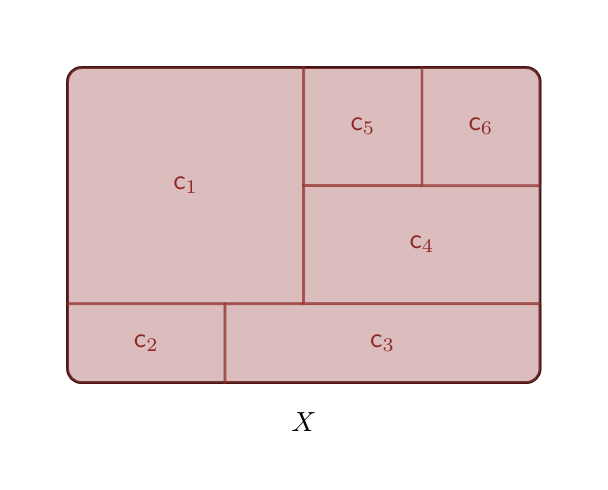
\begin{tikzpicture}[scale=1]
  \draw[white] (-0.5, -1) rectangle (6.5, 4.5);
  \draw[rounded corners=5, color=black, line width=1] (0, 0) rectangle (6, 4);
  \node at (3, -0.5) { $X$ };
  
  \filldraw[draw=dark, fill=mid, opacity=0.5, line width=1]
    (0, 1) -- (3, 1) -- (3, 4) {[rounded corners=5] -- (0, 4)} -- cycle;
  \node[dark] at (1.5, 2.5) { $\mathsf{c}_{1}$ };

  \filldraw[draw=dark, fill=mid, opacity=0.5, line width=1]
    (2, 0) -- (2, 1) -- (0, 1) {[rounded corners=5] -- (0, 0)} -- cycle;
  \node[dark] at (1, 0.5) { $\mathsf{c}_{2}$ };
  
  \filldraw[draw=dark, fill=mid, opacity=0.5, line width=1]
    (6, 1) -- (2, 1) -- (2, 0) {[rounded corners=5] -- (6, 0)} -- cycle;
  \node[dark] at (4, 0.5) { $\mathsf{c}_{3}$ };
  
  \filldraw[draw=dark, fill=mid, opacity=0.5, line width=1] (3, 1) rectangle (6, 2.5);
  \node[dark] at (4.5, 1.75) { $\mathsf{c}_{4}$ };
  
  \filldraw[draw=dark, fill=mid, opacity=0.5, line width=1] (3, 2.5) rectangle (4.5, 4);
  \node[dark] at (3.75, 3.25) { $\mathsf{c}_{5}$ };
  
  \filldraw[draw=dark, fill=mid, opacity=0.5, line width=1]
    (4.5, 4) -- (4.5, 2.5) -- (6, 2.5) {[rounded corners=5] -- (6, 4)} -- cycle;
  \node[dark] at (5.25, 3.25) { $\mathsf{c}_{6}$ };
\end{tikzpicture}

\end{document}  